% Figure: Llama-4 form sensitivity vs other LLMs.
\begin{figure}[t]
\centering
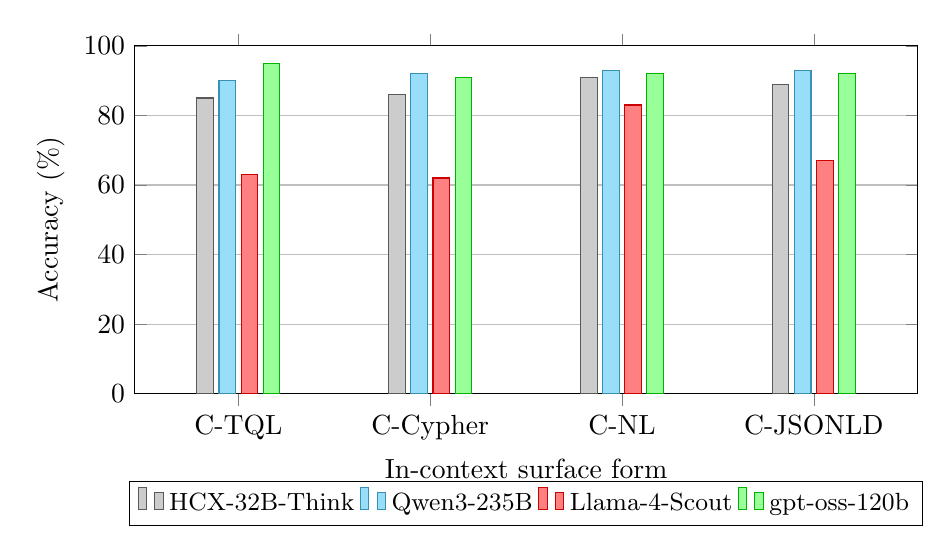
\begin{tikzpicture}
\begin{axis}[
  width=0.95\textwidth,
  height=6cm,
  ybar=2pt,
  bar width=6pt,
  ymin=0, ymax=100,
  ymajorgrids=true,
  ylabel={Accuracy (\%)},
  xlabel={In-context surface form},
  symbolic x coords={C-TQL, C-Cypher, C-NL, C-JSONLD},
  xtick=data,
  legend style={at={(0.5,-0.25)}, anchor=north, legend columns=4, font=\small},
  enlarge x limits=0.18,
]
\addplot[fill=gray!40, draw=gray!70!black] coordinates {
  (C-TQL, 85) (C-Cypher, 86) (C-NL, 91) (C-JSONLD, 89)
};
\addplot[fill=cyan!40, draw=cyan!70!black] coordinates {
  (C-TQL, 90) (C-Cypher, 92) (C-NL, 93) (C-JSONLD, 93)
};
\addplot[fill=red!50, draw=red!80!black] coordinates {
  (C-TQL, 63) (C-Cypher, 62) (C-NL, 83) (C-JSONLD, 67)
};
\addplot[fill=green!40, draw=green!70!black] coordinates {
  (C-TQL, 95) (C-Cypher, 91) (C-NL, 92) (C-JSONLD, 92)
};
\legend{HCX-32B-Think, Qwen3-235B, Llama-4-Scout, gpt-oss-120b}
\end{axis}
\end{tikzpicture}
\caption{In-context surface-form accuracy by LLM family. Three of four
LLMs are essentially form-agnostic (within 8 percentage points across
TQL, Cypher, NL, JSON-LD). Llama-4-Scout exhibits a 21-percentage-point
gap (C-NL 83\% vs.\ C-TQL/Cypher 62--63\%), tracing the bottleneck to
\emph{query-language familiarity in pretraining} rather than the
expressivity of the underlying KG.}
\label{fig:form-sensitivity}
\end{figure}
